\chapter{Evaluation\label{cha:evaluation}}
%4580
Throughout this thesis the requirements, design and prototype implementation of
the \ep~system that can support \LLLs has been discussed. This chapter focuses
on the evaluation of this research and its contributions based on three studies.
The studies were designed to look into the specific aspects of \LLLs support and
understand how well developed features satisfy the requirements identified
earlier by the lecturers and students. 

The number of studies represents perspectives of all of the stakeholders that
have been involved in this research earlier, i.e., lecturers and students.
Reason for this was to ensure that all of the perspectives are being captured as
\textit{different stakeholders often have different perspectives}
\citep[p.~111]{Hevner2010}. In addition, the evaluation from the students'
perspective has been split into two studies as the requirements elicitation
stage discovered that the perception of \LLLs depends on the maturity of
students. Therefore, it was decided to use different evaluation approaches for
each group of students.

The first section of this chapter describes the approaches and data collection
methods used in the evaluation stage. Further, each of the three studies is
presented with the detailed participants profile description, exercise protocol
followed by the study, artifacts collected and the results of data analysis.
Each study section ends with conclusions that look into recommended improvements
to the \ep~system prototype and its processes.

\section{Design Overview}
As this chapter aims to evaluate this research and its contributions, the
relevant research question and its sub-questions are restated here:

\textit{Does the extended environment meet the needs of the stakeholders in
university teaching and learning contexts?}

\textit{\begin{itemize}
  \item How can lecturers use new features to provide students with their
  guidance and help them to understand \LLLs skills?
  \item How can students address \LLLs skills using new features?
  \item How can new features help students track their learning progress, manage
  \ep~knowledge and content, demonstrate and share their achievements with
  others?
\end{itemize}}

To answer these questions, three studies were carried out independently from
each other. The results were used to evaluate the developed prototype from three
different perspectives: lecturers, mature students and less experienced
students. Each study followed its own exercise protocol described in the related
sections. Detailed design of each study can be found further in this chapter in
Sections \ref{sec:one}, \ref{sec:two}, and \ref{sec:three} respectively.

Data collection for analysis was performed using both quantitative and
qualitative methods to support the principles of multiple sources and multiple
perspectives of data advocated by many researchers
\citep{Yin2009,Maimbo2005,Marshall2010}. The following techniques were used over
the course of all studies:

\begin{itemize}
  \item Behavior observations made by the researcher during all studies.
  \item Observation data in form of digital photographs taken during the group
  experiments.
  \item Audio recordings of the face-to-face interviews collected to facilitate
  more thorough interview analysis.
  \item Open-ended questions asking for participants opinion on the features and
  tools used in the studies.
  \item Close-ended questions that required participants' evaluation based on
  ten point scale, from \textit{not useful at all} to \textit{highly useful}, 
  included in exit questionnaire.
  \item Physical artifacts in form of paper records made by participants of the
  group experiments.
  \item Digital artifacts in form of electronic records in the \ep~system made
  by participants of the groups experiments and case studies.
  \item System logs demonstrating \ep~system use by case study participants.
  \item Additional evidence, comments and opinions collected by the researcher
  through informal discussions that would help to support analysis and
  conclusions.
\end{itemize}

Audio recordings as well as digital photographs were collected with the
permission of the participants and performed without interrupting the process of
each study. More detailed description of data collection methods for each study
can be found in the relevant sections this chapter and associated appendices. 

\section{Ethical Considerations}

Similarly to the earlier stage of the requirements elicitation, the Massey
University Ethics Approval process was followed for the evaluation studies of
this research. Analysis of the evaluation design with the Human Ethics Chair
concluded that none of the three studies required full ethical approval.
Therefore, a ``Low Risk Notification" was submitted to the Massey University's
Low Risk Database.

Ethics documentation, such as the Ethics Approval Letter, lecturers and students
information sheets and participants' consent forms, used for this research
stage, can be found in Appendix \ref{cha:app5}.

\section{Study One. Exploratory Evaluation by Lecturers}
\label{sec:one}

To achieve the ultimate goal of this research project to develop a system that
can provide support for \LLLs in universities, it is important that learning
facilitators, e.g. lecturers, could successfully utilize improved technology to
help and guide students in their learning journey. Therefore, this study
explores the prototype implementations from the lecturers' perspective to
understand whether their initial requirements were met.

\subsection{Goals}

The goal for this study was:

\smallquote{To find out whether lecturers can use new features to provide
students with their guidance and support, and help them to understand \LLLs
skills.}

To support achievement of this goal the main objectives were:

\begin{itemize}
  \item To evaluate whether new features can provide better communication
  opportunities between lecturers and students;
  \item To determine how lecturers can use new features to help students
  understand the link between \LLLs skills and their university degree study;
  \item To explore how lecturers can utilize new features in the classroom to
  guide students through development of \LLLs skills. 
\end{itemize}

\subsection{Research Protocol}

This study was an exploratory study that used a demonstration and participants
interviews as a research evaluation approach. According to \citet{Peffers2008},
\textit{demonstration} is normally used to show that idea works and precedes a
more \textit{formal} evaluation. Here, demonstration was included into the
overall evaluation design. The expectation was that in combination with the
participant interviews it would provid a valuable insight into the lecturers'
perspective on the prototype features.

For the purpose of this study, six personal and one small group interviews were
organized with the participants. Group interview was undertaken during the
annual staff meeting and involved three participants.

This study did not follow a strictly defined research protocol as the directions
of the meeting discussions were based on the outcomes of the semi-formal
conversations with the participants. To guide the course of the study, the
researcher initially had a set of topics to cover in the presentation and
demonstrate the prototype functionality with the examples of how it could be
potentially adopted in the learning environment. The discussion topics were
based on the implemented features described in detail earlier in Chapter
\ref{cha:prototype}.

Each of the topics was presented to the participants in the following order:

\begin{itemize}
  \item the problem addressed in the topic;
  \item an implementation suggested to solve the problem;
  \item a step-by-step demonstration of how this implementation works in the
  \ep~system;
  \item expected/intended use of the feature in the classroom;
  \item where possible, provide examples of use in the \ep~system.
\end{itemize}

After the demonstrations, the participants were asked to assess the prototype
features based on their personal and professional experience. From their
perspective they evaluated whether the presented scenarios of use were realistic
and what challenges they could see in the suggested ways of using the features.

The lecturers were then asked to suggest how they would use new features and how
they would apply the methods these features incorporate with their students. At
the end of the topic discussion, the participants were offered to recommend the
potential improvements.

All interviews were audio recorded and transcribed for the purpose of more
thorough analysis. 

\subsection{Participants Profile}

This study used a number of techniques to identify suitable participants.
Initially, each of the lecturer-participants of the previous stage of
identifying requirements for \LLLs supported by \ep~systems was offered to take
part in the evaluation of the prototype implementations at the later stages of
this research. Three lecturers expressed interest in continuing their
participation in the project.

The rest of the participants were recruited using snowball sampling strategy
which had already been employed earlier in this research. This strategy relied on
recommendations of the existing participants having knowledge of the suitable
candidates who would potentially be interested in this research. Based on
criteria of being a lecturer or having previous lecturing experience, and
also having experience of using an \ep~system with the students, six other
participant were identified from the suggested candidates.

Overall, the data was gathered from nine participants, all lecturers at
various schools and colleges of Massey University. Table \ref{tab:study1part}
shows demographics of the participants:

\begin{table}[htb]
  \begin{center}
    \begin{tabular}{| l | c |}
    \hline
     \multicolumn{1}{|c|}{\textbf{University Structure}} &
     \multicolumn{1}{c|}{\textbf{Number}} \\ \hline
		College of Science: & \\ 
		-- School of Engineering and Advanced Technology & 1 \\
		-- Institute of Veterinary, Animal and Biomedical Sciences & 1 \\
		-- Institute of Food, Nutrition and Human Health & 1 \\ \hline
		College of Education: & \\ 
		-- School of Curriculum and Pedagogy & 2 \\
		-- School of Educational Studies &  3 \\ \hline
		Centre for Teaching and Learning & 1 \\ \hline
	\end{tabular}
  \end{center}
\caption{Demographics of the Study One participants (n = 9)}
\label{tab:study1part}
\end{table}

One of the participants was a program coordinator for a Bachelor degree program
and had a particular interested in how the prototype functionality can be used
with the university graduate attributes and \LLLs skills.

The lecturers from the College of Education had the most experience of using
portfolios or \ep s with their students. The reason for this was that every
potential teacher in New Zealand had to meet the requirements developed by the
New Zealand Teachers Council in form of Graduating Teacher
Standards\footnote{\url{http://www.teacherscouncil.govt.nz/te/gts/}}. These
standards closely resemble university graduate attributes and \LLLs skills.
Teaching portfolio has to created by students as a proof that they meet these
standards. The College of Education lecturers were at the earlier stages of
adoption the \ep~system for these purposes and therefore were highly interested
in giving their feedback on the prototype implementations.

A representative of the Centre for Teaching and Learning was considered a
suitable participants as they had previous teaching experience, both at school
and at university, and at that time was assisting adoption of the new learning
technologies, \ep~systems in particular, in the university courses.

Each participant was approached by an invitation email to take part in this
research and evaluate the developed features in a face-to-face meeting with the
researcher.

\subsection{Results}

Students could use it for various reasons: to communicate what they've learnt
to somebody else or to try to make sense of the things that they are learning
right now.

so that at the end they can clearly understand how everything is built towards
them achieving these attributes or not.

The problem from the lecturer's perspective is that students are less likely to
use the system \textit{``for their own good''}. Therefore, it might require an
element of assessment. However, if it needs to be assessed, than it becomes an
exercise that requires to be completed which is not the same thing as using
system on their own motivation.

Jane: Our challenge is to develop this notion of lifelong learning ability and
what it means for that to be a good practicing engineer. And we need to embed it
early on, because they [students] don't know the notion at the moment.

It might not be the right way, but it could be the way that would help us do
it, rather than start from scratch.

I would be interested in the students try to use this tool and how they see that
and is this a viable tool. Are they going to keep using it?

I can see some opportunities for what we are trying to do in the future. I
definitely see potential. At the moment, I an not sure how I would apply it, we
need to try.

The driver here is that you are going to go out there and demonstrate that you
can contribute to an organization and what is it that you are taking from your
experience of learning. And it's not necessarily technical knowledge, it's all
the other stuff.

What I like about that, I am looking for both horizontal integration of what
they are learning from other papers as 

What they liked:
- Visual nature of concept mapping
- simplicity of making complex things
- challenge of conceptual understanding
- authentic evidence that students meet the outcomes

Potential challenges:
- training of lecturers as well as students 
- assistance throughout the entire process
- 

\subsection{Conclusions}

Overall, the outcomes of Study One were very useful and provided valuable
first-hand evidence reaffirming that the lecturers' requirements of the earlier
project stage implemented in the prototype were met.

Based on discussions during the demonstrations and the interviews with
participants afterwards, it can be concluded that the prototype features were
well accepted and raised an interest.

After the formal part, five out of nine participants asked when they could
expect to see the demonstrated features in the official release of the
\ep~system that they had been using in the university and expressed willingness
to include these into their work with students. Arguably, this can be considered
as an indicator of value and usefulness of the developed features recognized by
the participants during the demonstration.

\section{Study Two. Group Experiment -- \LLLc Skills Development and
Demonstration}
\label{sec:two}

This study investigates students perception of the concept mapping tools as a
part of the \ep~system in terms of constructing and sharing knowledge,
understanding and demonstrating achievements, and linking practical experiences
to the conceptual skills.

\subsection{Goals}
The goal for this study was:

\smallquote{To find out whether undergraduate students find concept mapping embedded
into the \ep~system helpful in terms of addressing graduate attributes, learning
objectives and \LLLs skills and tracking their progress in learning.}

To support achievement of this goal the main objectives were:

\begin{itemize}
  \item Determine whether concept mapping embedded into the \ep~system provides
  students with a suitable tool for addressing graduate attributes and \LLLs
  skills;
  \item Investigate whether developing of concept maps influences students'
  understanding of personal learning achievements and skills that they develop
  during degree program study;
  \item Determine whether concept mapping embedded into the \ep~system can be
  successfully used to demonstrate personal achievements and skills;
  \item Analyse how useful students' consider concept mapping methods as a part
  of the \ep~system.
\end{itemize}

\subsection{Research Protocol}

To ensure a better control over experiment settings, it was conducted with the
small groups of students at a time (35 participants in total). All groups
followed the similar process outlined in Study Protocol in Appendix
\ref{cha:app6} with up to two hours for the entire experiment to complete. Time
of completion might have varied between groups due to the differences of
participants' previous experiences. For example, some of the students did not
require explanation of \LLLs concepts or tutorial on how to construct concept
maps.

Work with each group of students began with an introduction to the research,
activities to be performed and an explanation of participants' rights.
Ethics documents, such as the information sheet and consent form, were
distributed. Signed consent forms to participate in the experiment had been
collected before any other activities and exercises were started.

The introduction included a brief overview of the research project, a
presentation on \LLLs concepts, demonstration of the \ep~system and concept
mapping as a method of constructing knowledge.

After introduction part, each participant received pen and paper to work with
the first exercise, examples of institutional attributes and courses learning
objectives, examples of concept maps, unique access account to the prototype
\ep~system, user manual for the \ep~system concept mapping tool and artifacts
fragments extraction, and exit questionnaire.

Second part of the experiment consisted of two exercises: the first one
performed on paper and the second one performed using the \ep~system tools.
Between the exercises, students were given a demonstration of the prototype
functionality that allowed to construct concept maps in the \ep~system and
attach examples from the \ep~repository to the concepts. After the
demonstration, students proceeded to the second exercise. At the end, all
participants were asked to complete the exit questionnaire to collect their
opinion on the tools and methods they had just used.

\begin{figure}[htb]
\centering
\includegraphics[width=1\textwidth]{CH7-F7-Settings}
\caption{Experiment settings}
\label{fig:settings}
\end{figure}

Figure \ref{fig:settings} shows the settings in which the experiment was
performed. Standard university computer classrooms were used for the experiment.
Participants did not have allocated places which allowed them to choose more
comfortable settings for the duration of the experiment. The researcher was
available at any time during the experiment for assistance.

Although, working independently during the experiment was highly encouraged,
students were allowed to do exercises in pairs or groups up to three students.
In case they were working in pairs, students still had to complete the exit
questionnaire independently.

\FloatBarrier

\subsection{Participants Profile}

As it was already mentioned in the previous section, thirty five students from
various undergraduate programs at Massey University agreed to participate in
this experiment. Table \ref{tab:degree} shows the wide range of degree programs
the students were enrolled in.

\begin{table}[htb]
  \begin{center}
    \begin{tabular}{| l | c |}
    \hline
     \multicolumn{1}{|c|}{\textbf{Degree Program}} &
     \multicolumn{1}{c|}{\textbf{Number}} \\
     \hline
     Bachelor of Engineering & 2 \\ \hline
     Bachelor of Health Science & 1 \\ \hline
     Bachelor of Science & 3 \\ \hline
     Bachelor of Veterinary Science & 7 \\ \hline
     Graduate Diploma in Secondary Teaching & 14 \\ \hline
     Graduate Diploma in Primary Teaching & 7 \\ \hline
     Bachelor of Information Sciences & 1 \\ \hline
    \end{tabular}
  \end{center}
  \caption{Degree programs of the Study Two participants (n = 35)}
  \label{tab:degree}
\end{table}

All participants were volunteers recruited through the announcements in the
classroom of various courses in College of Education and College of Science or
through the poster invitation distributed through the lecturers at Massey
University.

As shown in Figure \ref{fig:demograph}, participants' age ranged largely from
twenty to thirty years which was expected as this experiment aimed on studying
undergraduate students. Gender distribution was relatively equal with fifteen
male and twenty female participants.

\begin{figure}[htb]
\centering
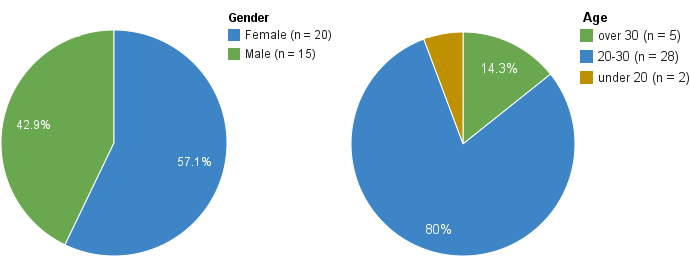
\includegraphics[width=1\textwidth]{CH7-F5-Demographics}
\caption{Participant demographics (n = 35)}
\label{fig:demograph}
\end{figure}

Twenty seven students reported that they were familiar with the concepts
of \LLLs before the experiment. However, only thirteen of these twenty seven
students said that they were familiar with the term \textit{graduate
attributes}. They were primarily Teaching Diploma students. As it was discovered
in informal post-experiment discussion, this might be explained by the fact that
College of Education of Massey University uses term \textit{teaching profile}
instead of \textit{graduate attributes} to describe \LLLs skills and
competences.

In the background section, twenty nine students said that they knew about
\textit{\ep} prior to the experiment. Seven of these students reported using an
\ep~system to demonstrate their \LLLsn. They were Veterinary Science students
who had \ep~work included into their degree program curriculum.

\subsection{Activities and Artifacts}

Figure \ref{fig:procedure} provides an overview of the experiment procedure and
the activities or tasks performed for each part based on the study protocol.

\begin{figure}[htb]
\centering
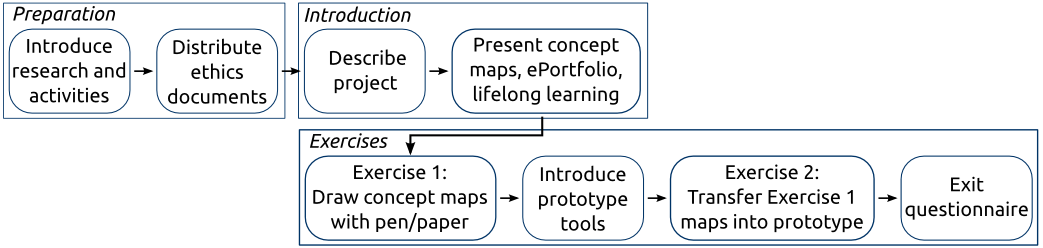
\includegraphics[width=1\textwidth]{CH7-F8-Activities}
\caption{Experiment procedure}
\label{fig:procedure}
\end{figure}

Length of the presentations and information content of the introduction part
varied depending on the participants' experience.

List of the artifacts used by the students in this experiment was following:

\begin{itemize}
  \item Ethics documents: a) information sheet, and b) consent form;
  \item Pen and paper for the first concept mapping exercise;
  \item Examples of institutional attributes and courses learning objectives
  taken from the Massey University web-site;
  \item Examples of concept maps in the \ep~system created by the researcher;
  \item Instruction sheet with the unique access account to the \ep~system;
  \item User manual for the \ep~system concept mapping tool;
  \item User manual for artifacts fragments extraction;
  \item The exit questionnaire.
\end{itemize} 

Appendix \ref{cha:app6} provides samples of documents used in the experiment.
Participants' responses from the exit questionnaire can be found in Section
\ref{sec:responses} of this appendix.

\subsection{Data Analysis and Results}

The data collected during this evaluation were based on questionnaire results,
observations and system records. These are described in the related subsections
of this section.

\subsubsection{Observed Behaviour}

Based on observations, the most difficult for students was the very beginning of
each of the exercises. In the informal discussion after the experiment, some
of the students admitted that having a blank sheet of paper or an empty
\ep~system account in front of them as they started was rather intimidating. At
first, students expected to be told what to draw and which concepts to include
into their diagrams. After a short explanation that there were no right or wrong
concept maps that could represent their own learning experience or skills, the
process of working with concept maps moved on.

All students were able to complete exercises in allocated time. Students, new to
the concept mapping, followed the techniques presented in the introduction
tutorial on how to build the maps. This included deciding the main message or
key concept of their map followed by identifying the related concepts. When this
was done, they tried to organize the concepts into maps.

% TODO: photo of the concept map on paper
\note{TODO: Add photo of maps on paper here}

More experienced students preferred to follow their own established procedure of
creating concept maps. Some of them did not spend time making a list of the
concepts, but were adding concepts straight to the maps making corrections when
necessary.

Due to the lack of information about previous experiences of the participants,
in some cases groups consisted of students with very different knowledge of the
discussed concepts. The problem with this situation was that while the students
with no experience required assistance, more experienced participants tended to
jump ahead of the group in doing exercises, following manual on their own and
not waiting for the demonstration of the evaluated functionality of the
prototype. At this stage, it is not possible to analyse whether this had any
influence on the results of the evaluation, as the demonstration which those
students would have followed, had the same information content as the user
manual on the prototype functionality. Therefore, it possible to assume here
that all participants worked under the same conditions.

\subsubsection{Exit Questionnaire Results}
The exit questionnaire responses were the major data collection source for the
user feedback and evaluation.

In general, the responses were very positive. Comments made by the participants
during the exercises showed that they enjoyed the work with concept mapping
tools in the \ep~system.

Based on the responses to the Section B of the exit questionnaire, students
found \ep~concept mapping to be a valuable experience. According to their
comments, the tools and methods that were used during the experiment helped
them to think about bigger picture of their learning, make links between the
concepts they have learnt at the university, think how these concepts contribute
to the skills development, and organize their previous experience in a 
structured way that could be shared with others.

In the informal conversation after the experiment, a number of students asked
for permission to keep the \ep~system login information they have been provided
with for the time of the study in order to use it later on their own. Although,
these students have not been rejected in the system access, they were warned
that the \ep~system was going to be fully supported only for the duration of the
research project. From the perspective of the research evaluation, this
expression of interest can be considered an additional measure of success of the
tools used by the students.

Table \ref{tab:study2summary} summarizes the overall participants experience of
using concept mapping in the \ep~system. The number in brackets indicates the
number of participants who mentioned these features in their responses. In
some cases one student could name more that one feature they liked or not
mention anything at all.

\begin{table}[htb] \small
  \begin{center}
    \begin{tabular}{| p{6.5cm} | p{6.5cm} |}
    \hline
     \multicolumn{1}{|c|}{\textbf{Most favoured part/feature}} &
     \multicolumn{1}{c|}{\textbf{Least favoured part/feature}} \\
     \hline
     Ease of use (11) & Complicated to add examples (6) \\ \hline
     Extracting fragments (7) & Might be time consuming (6) \\ \hline
     Visual representation of knowledge (7) & Might be difficult without initial help (4) \\ \hline
     Link between concepts and experience (5) & Restricted maps formatting (2) \\ \hline 
     Sharing of development (4) & Restricted examples format (1) \\ \hline
     Tracking progress (4) & Learning system is complex (1) \\ \hline
     Shows bigger picture (3) &  \\ \hline
     Targeted reflection (2) & \\ \hline
     Gets the thinking process going (1) & \\ \hline
    \end{tabular}
  \end{center}
  \caption{Participants' feedback on the concept mapping in the \ep~system }
  \label{tab:study2summary}
\end{table}

Examples of responses to the Section B of the exit questionnaire can be found in
Section \ref{sec:responses} of Appendix \ref{cha:app6}.

At the end of the exit questionnaire, the participants were asked to evaluate
usefulness of the used tools based on ten point scale where ten points
represented \textit{highly useful} score and one point represented \textit{not
useful at all} score. Chart \ref{fig:overall} shows the overall scores based on
participants responses.

\begin{figure}[htb]
\centering
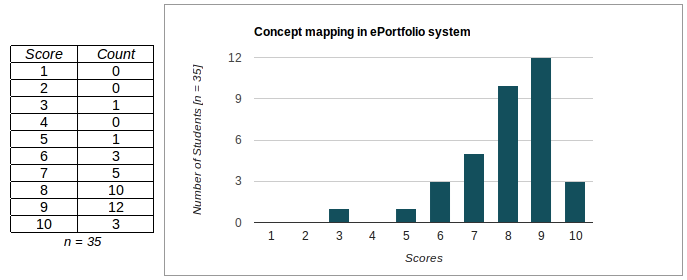
\includegraphics[width=1\textwidth]{CH7-F1-Chart}
\caption{Overall views on usefulness of the used tools and methods}
\label{fig:overall}
\end{figure}

The questions that can be asked here is whether participants' previous
experience with either \ep s systems or familiarity with the \LLLs concepts
influenced the perception of usefulness of the concept mapping tool as a part of
the \ep~system.

For this purpose, the results were split into three groups (Figure
\ref{fig:groups}) based on the differences in participants' experience
reported in the background section (Section A) of the exit questionnaire:

\begin{figure}[htb]
\centering
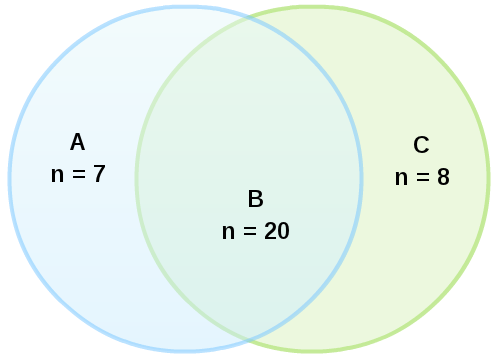
\includegraphics[width=0.5\textwidth]{CH7-F6-Groups}
\caption{Experiment groups based on student profiles}
\label{fig:groups}
\end{figure}

\FloatBarrier

\textit{Group A} represents participants who were familiar with the concepts of
\LLLs prior to the experiment. \textit{Group C} consists of students who have
not been using any kind of \ep~system to demonstrate their \LLLs prior to the
experiment. \textit{Group B} represents an intersection of groups A and C and
therefore consists of students familiar with \LLLsn, but who have not been using
\ep~systems. In this case, \textit{Group A} also represents students who
have used an \ep~system for \LLLs purposes prior to the experiment. Variable
\textit{n} represents a number of participants in each group respectively.

According to such distribution of the participants into groups, the views on
usefulness of the \ep~system concept mapping tools were following:

\begin{figure}[htb]
\centering
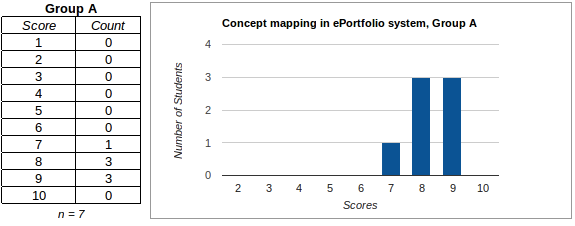
\includegraphics[width=1\textwidth]{CH7-F2-Chart-GA}
\caption{Group A views on usefulness of the used tools and methods}
\label{fig:group1}
\end{figure}

\begin{figure}[htb]
\centering
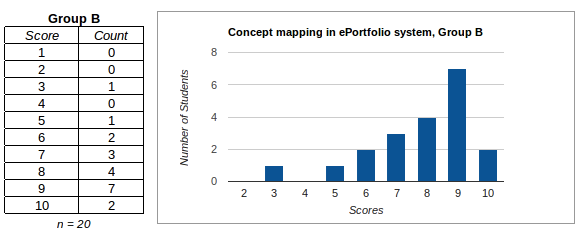
\includegraphics[width=1\textwidth]{CH7-F3-Chart-GB}
\caption{Group B views on usefulness of the used tools and methods}
\label{fig:group2}
\end{figure}

The student from Group B (Figure \ref{fig:group2}) who gave three points to the
usefulness score of the used tools decided not to justify their choice by the
exit questionnaire responses. The only comment they left was \textit{``You can't
quite do what you want with it''} without an overall experience description,
recommended improvements, or description of the least favoured parts.

\begin{figure}[htb]
\centering
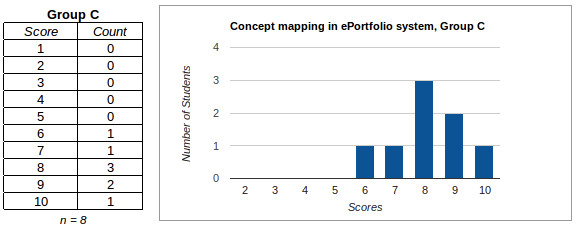
\includegraphics[width=1\textwidth]{CH7-F4-Chart-GC}
\caption{Group C views on usefulness of the used tools and methods}
\label{fig:group3}
\end{figure}

\FloatBarrier

In general, it can be seen that participants of all groups gave high scores as a
measure of usefulness of the concept mapping tools in the \ep~system they had used. It can
be also concluded that the previous experience with the overall concepts did not
have substantial influence on the score distribution. However, it must be
noticed that Group B (Figure \ref{fig:group2}) has a significantly larger number
of students compared to Groups A (Figure \ref{fig:group1}) and C (Figure
\ref{fig:group3}). Nevertheless, the conclusion drawn from this analysis can be
that the novice users find the tools that had been used during the experiment
the same useful as the students familiar with either one or both concepts of
\LLLs and \ep s.

\subsubsection{Concept Maps Created by Students in the \ep~System}

Section \ref{sec:examples1} of Appendix \ref{cha:app6} provides examples of the
concept maps created by the students during the experiment. As it was
requested by the exercise task, the majority of students transferred their hand
drawn concept maps to the \ep~system. A small number of concepts had examples
attached to them that would demonstrate students' experience of the related
concepts. Due to the fact that the participants had not been expected to bring
examples with them to the study, they were asked to think about what examples
they would include and create empty files or short blog posts for these. As it
was explained to the students, understanding and evaluation of the general
concept rather than content they create was in focus of this study.

\subsection{Conclusions}

Overall, it can be concluded that the fundamental goal of this study to
evaluate whether the students find prototype tools helpful was accomplished. It
showed that students perception of the concept mapping as a part of the
\ep~system was positive and it provided a suitable means of addressing graduate
attributes and \LLLs skills.

Students who have had prior experience with using the \ep~system to demonstrate
their \LLLs skills said that concept mapping was a great idea and worked better
for them than the \ep~tools they had used before.

Although, usability was not in focus of the prototype requirements, a large
number of students noticed that concept mapping was easy and straightforward to
use. In contrast, extracting fragments of the artifacts and adding them as
examples to the concepts was more complicated and less intuitive task and
required detailed instructions. However, a common agreement among the
participants was that with proper training and experience all tasks can be
easily performed on daily basis.

A problem with the participants testing software rather than evaluating the
overall method and its concepts was expected to be a potential threat for
the outcomes of this study. For this reason, in the introduction part of the
experiment it was emphasized that the participants were going using prototype
functionality and therefore should not pay attention to the flaws of the user
interface, but focus on the process and an overall idea. Unfortunately, it was
impossible to avoid the responses that indicated that participants were looking
at the software and its functionality instead trying to understand what stands
behind it. This could be seen in such comments like \textit{``Date format on the
page is not right for New Zealand''}, \textit{``I would like to have a choice of
color boxes''}, or \textit{``Bigger, more approachable toolbar would be nice''}.
However, there were no more than four responses similar to these for each
question.

Among the improvements suggested by the participants were:

\begin{itemize}
  \item Simplification of the process of linking examples to the concepts
  \item Improved maps formatting and reorganizing options for higher
  flexibility of the concepts and better delivery of owners message
  \item Video tutorial and more detailed instructions on using concept mapping
  tools to ensure that even novice users can start on their own without external
  help
  \item Options of linking items outside of the \ep~repository to bring other
  sources of learning to the \ep~system
  \item More examples of the concept maps for students with various profiles --
  resembles the need of providing the students with a model \ep~example
\end{itemize}

These recommendations can be used to desing further improvements to the process
and the overall concept to ensure that they are accepted by the students with
diverse level of experience.
 
\section{Study Three. System Validation by Experienced Students}
\label{sec:three}

This section

\subsection{Goals}

The goal for this study was to

\subsection{Research Protocol}

Appendix \ref{cha:app7}.

\subsection{Participants Profile}

Case studies are commonly used as evaluation method \citep{Yin2012}

 Strategy used to identify suitable cases. According to \citet{Stake1995},
 while selecting cases researchers should try to keep a balance between the
 uniqueness and the ordinariness.

Maximum variation cases \citep{Flyvbjerg2006}: cases were different in
one dimension: experience with using \ep~system.

\subsection{Activities and Artifacts}



\subsection{Data Collection and Analysis}

Face-to-face interview, system logs, cmaps, artifacts uploaded to the system.

They all viewed the prototype implementations positively.


\subsection{Conclusions}

It can be concluded

Overall, based on the evidence, it can be conclused that all three participants
supported the prototype implementations and agreed that being properly untilized
these implementations could be a part of a successful approach to \LLLs support
in universities.
 
\section{Summary}

This section presented the evaluation design and the results of the evaluation
of the contributions of this research project.
